\chapter{Projektafgrænsninger}
Dette kapitel beskriver projektets afgrænsninger og hvilke arbejdsopgaver der er frasorteret i udviklingsfasen. Afgrænsninger kan både være helt undladt i projektet, eller bestemte faktorer der har begrænset udvikling af visse dele i systemet. 

\section{Sikkerhedskontrol} \label{title:sikkerhedskontrol}
Fra projekts start, i forprojektet, lå der et ønske fra kundens side omkring en sikkerhedskontrol ved konditioneringsbehandlingen. Fra kundens side bestod ønsket i at kontrollere kredsløbet på patienten, der modtog konditioneringsbehandling. Ønsket lød på at bruge et pulsoximeter som sikkerhedskontrol. Det færdige produkt skulle ved hjælp af et pulsoximeter kontrollere patients saturation og puls og ud fra threshold værdier vurdere om patienten kunne tåle behandlingen. De tænkte cases, hvor sikkerhedskontrollen skulle afbryde behandlingen, var ved patienter med dårligt kredsløb, som under behandlingen udvikler koldbrand i den afklemte ekstremitet. Problematikken ved at bruge et pulsoximeter som sikkerhedskontrol, ligger i teknikken bag pulsoximeteri. 

Pulsoximeteri måler variationer i det pulserende blod ved at detektere ændringerne i absorption af lys fra to eller flere lyskilder med forskellige bølgelængder. Når væv belyses kan absorptionsgrundlaget opdeles i fire dele (Se figur \ref{fig:opticTissue})
\begin{figure}[H]
	\centering
	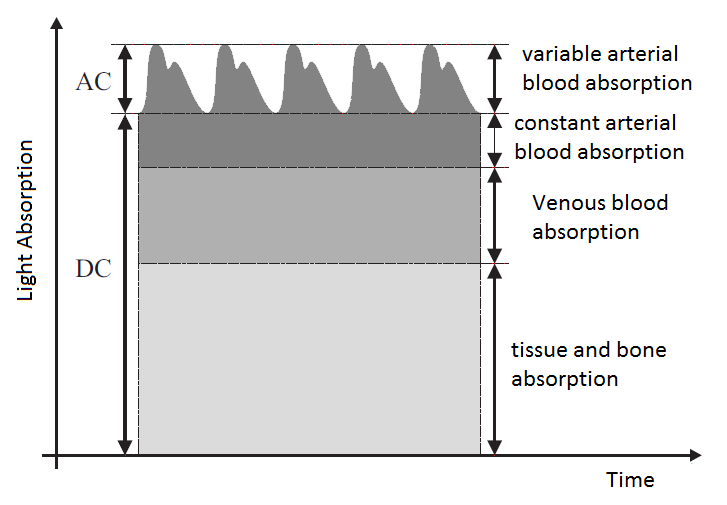
\includegraphics[width = 0.7\textwidth]{billeder/opticTissue.png}
	\caption{Oversigt over absorption af lys i væv}\label{fig:opticTissue}
\end{figure}

I pulsoximeteri filtreres alt DC væk; dvs absorption fra venøst blod, den konstante mængde af arterielt blod, samt alt andet væv. Det tilbageværende signal, er det pulserende arterielle blod. For at måle saturationen udregnes forskellen på absorption ved \textit{pulstop} og \textit{pulsbund}. Disse absorptioner kan ved hjælp af den molære extinction koefficient for hhv. oxyhæmoglobin og deoxyhæmoglobin og afstanden mellem lyskilde og modtager omregnes til relative koncentrations ændringer i hhv. oxyhæmoglobin og deoxyhæmoglobin. Disse relative koncentrations ændringer kan så omsættes til saturation via formlen \ref{eq:satequation}
\begin{equation}
	SaO_2 = \frac{\Delta[HbO_2]}{\Delta[HbO_2]+\Delta[HHb]} *100\%
	\label{eq:satequation}
\end{equation}

Efter som at pulsoximetri kun giver indblik i iltmætningen af det pulserende arterielle blod, indeholder den målte iltmætning ikke information angående det lokale væv, men kun information angående respirationen. Pulsoximeteri er derfor en indikator for respirationen og for hvor godt patientens respiratoriske kredsløb ilter blodet. Apopleksi patienter har som udgangspunkt ikke dårlig respiration, og saturationen af blodet vil derfor ligge over 90\%. Sikkerhedskontrollen skulle kontrollere om iltreserven i armen var nået op på et tilstrækkeligt niveau efter hver afklemning, men eftersom at saturationen ikke er et udtryk for vævet/statisk-blod (iltreserven i armen) kan pulseoximetri ikke måle iltreserven.
Det er heller ikke muligt, at måle AC værdier for det arterielle blod under en afklemning, fordi det pulserende signal ikke er tilstedeværende på grund af okklusionen. Derfor kan selv en person med dårlig kredsløb få målt normal puls og saturation, og stadig tage skade af konditioneringsbehandlingen. 

Denne problemstilling blev opdaget forholdsvis hurtigt i projektforløbet og kunden blev orienteret omkring problemstillingen. Det blev derfor bestemt at projektet skulle afgrænses i forbindelse med sikkerhedskontrollen. Der er gjort plads i udviklingsdokumentationen til implementering af en anden form for sikkerhedskontrol. For at få underbygget påstanden omkring pulsoximeteri og sikkerhedskontrol, har projektgruppen blandt andet været i kontakt med Troels Johansen, PhD studerende, fra lungemedicinsk afsnit på AUH (Se afsnit \ref{title:samarbejdspartnere} omkring samarbejdspartnere og mødereferat \ref{app:troelsuge40}). Troels kunne kun bekræfte påstanden omkring at pulsoximeteri som værende ugyldig til sikkerhedskontrol, og så i stedet muligheder i NIRS(Se afsnit \ref{title:nirs} i perspektivering) eller at bruge pulsoximeteri som kontrol af om afklemningen var tilstrækkeligt, pga. af den manglende puls ved totalt okklusion.

\section{MR kompatibilitet}
I forbindelse med forprojektet var et ønskescenarie fra kundens side, at apparatet, der skulle udvikles til at udføre konditionering, skulle kunne gå i en MR-scanner. Dette var et ønske, fordi perkonditionering, hvis det køres i fx 4 cyklusser af 5 minutter, vil tage længere tid at gennemfører, end den tid det ville tage at køre til hospitalet. Proceduren for patienter, der mistænkes for have apopleksi, er at få dem i MR scanneren så hurtigt så muligt. Derfor kan man i nogle tilfælde være nød til at afbryde konditioneringsbehandlingen og i den sammenhæng kan sætte spørgsmålstegn ved den gavnlige effekt RIC. Det blev meget hurtigt bestemt at projektet måtte afgrænse sig fra MR kompatibel, da dette ville stille alt for høje krav til produktets komponenter og dens håndtering af de ekstremt kraftige elektromagnetiske felter.

\section{Seagull samarbejde}
I begyndelsen af projektet blev der igennem kunden etableret et samarbejde med \textit{Seagull}, en dansk virksomhed, som skulle fungere som talerør til en kinesisk blodtryksapparat producent (Se afsnit \ref{title:samarbejdspartnere} omkring samarbejdspartnere). Tanken bag samarbejdet var at den kinesiske virksomhed skulle levere komponenter og teknisk sparring. Den danske virksomhed var med som mellemmand efter eget ønske, da den kinesiske virksomhed var deres kontakt. Et andet argument for virksomhedssamarbejdet, var et ønske fra kundens side omkring produktet skulle lige sig tæt opad Seagulls eksisterende apparater. 

Men efter flere forgæves forsøg på at kommunikere og få information ud af den kinesisk virksomhed, blev det opgivet at produktet skulle ligge sig op af deres apparater. Det forgæves samarbejde betød også at alt arbejdet med \textit{konditioneringsapparatet}, og især udviklingen af en blodtryksalgoritme måtte foretages på egen hånd af projektgruppen selv og uden nogen form for teknisk sparring. 

\subsection{Tavshedspligt} \label{title:tavshedspligt}
Pga. af patentundersøgelser har hele projekt været underlagt tavshedspligt og underskrevet tavshedserklæringer med både universitet og neurologisk afsnit. Tavshedspligten har bla. forsinket nogle processer da alle parter skulle have underskrevet en tavshedserklæring inden. I andre tilfælde hvor et samarbejde har været kortvarig eller der ikke har været tid til at underskrive tavshedserklæring, har projektgruppen måtte undlade detaljer ved kommunikation med disse samarbejdspartnere. Dette har i nogle tilfælde betydet at hjælpen fra evt. eksperter har været begrænset af manglende forståelse for projektet.  Derfor har de igangværende patentundersøgelser været en begrænsning for projektarbejdet i flere sammenhænge (Se tavshedserklæring \ref{app:tavshedserkl}).
Tavshedspligten har også betydet at der skulle tages bestemte hensyn i forbindelse med versionsstyring. Ved brug af git (Se afsnit \ref{title:versionsstyring} omkring versionsstyring) som versionsstyrings værktøj, har gruppen skulle betale for at få et private repository. Dette er normal gratis, men så er ens repository offentligt tilgængeligt.

\newpage
\section{Prototypen}
I dette afsnit beskrives hvilke beslutninger, som er truffet med begrænsende effekt på prototypen.

\subsection{Arduino}
\begin{minipage}[t]{0.6\textwidth}
På grund af projektets fokus på udvikling af en prototype, blev der truffet nogle valg i den indledende projektfase, med henblik på at øge udviklingshastigheden og sikre en høj fleksibilitet under udviklingen. Det blev derfor besluttet at anvende \textit{evaluation boards} i form af arduino til dette projekt(se figur \ref{fig:arduinoMega2560}), som netop er let tilgængelig og brugt i vid udstrækning til udviklingsprojekter. Arduino'en er støttet op omkring af et stort fællesskab, som giver gode support muligheder, samt biblioteker til et stort udvalg af shields. Alt dette giver anledning til en god start på projektet.\\

Arduino'en er et open source projekt, og alle komponenter og schematics er derfor frit tilgængelige, hvilket giver mulighed for at designe et endeligt fabrikations klart produkt ud fra konditioneringsapparatets prototype.\\

Desværre medfølger der også flere ulemper ved brug af arduinoen. Arduino'ens mangler, som særligt har begrænset dette projekt, er som følger:\\

\begin{itemize}
	\item Lav mængde RAM (Kun 8 KB) 
	\item 10bit ADC
	\item Microcontrolleren (ATmega2560)
\end{itemize}
Kilde: \cite{RefWorks:40}

\end{minipage}
\begin{minipage}[t]{0.4\textwidth}
	\begin{figure}[H]
		\centering
		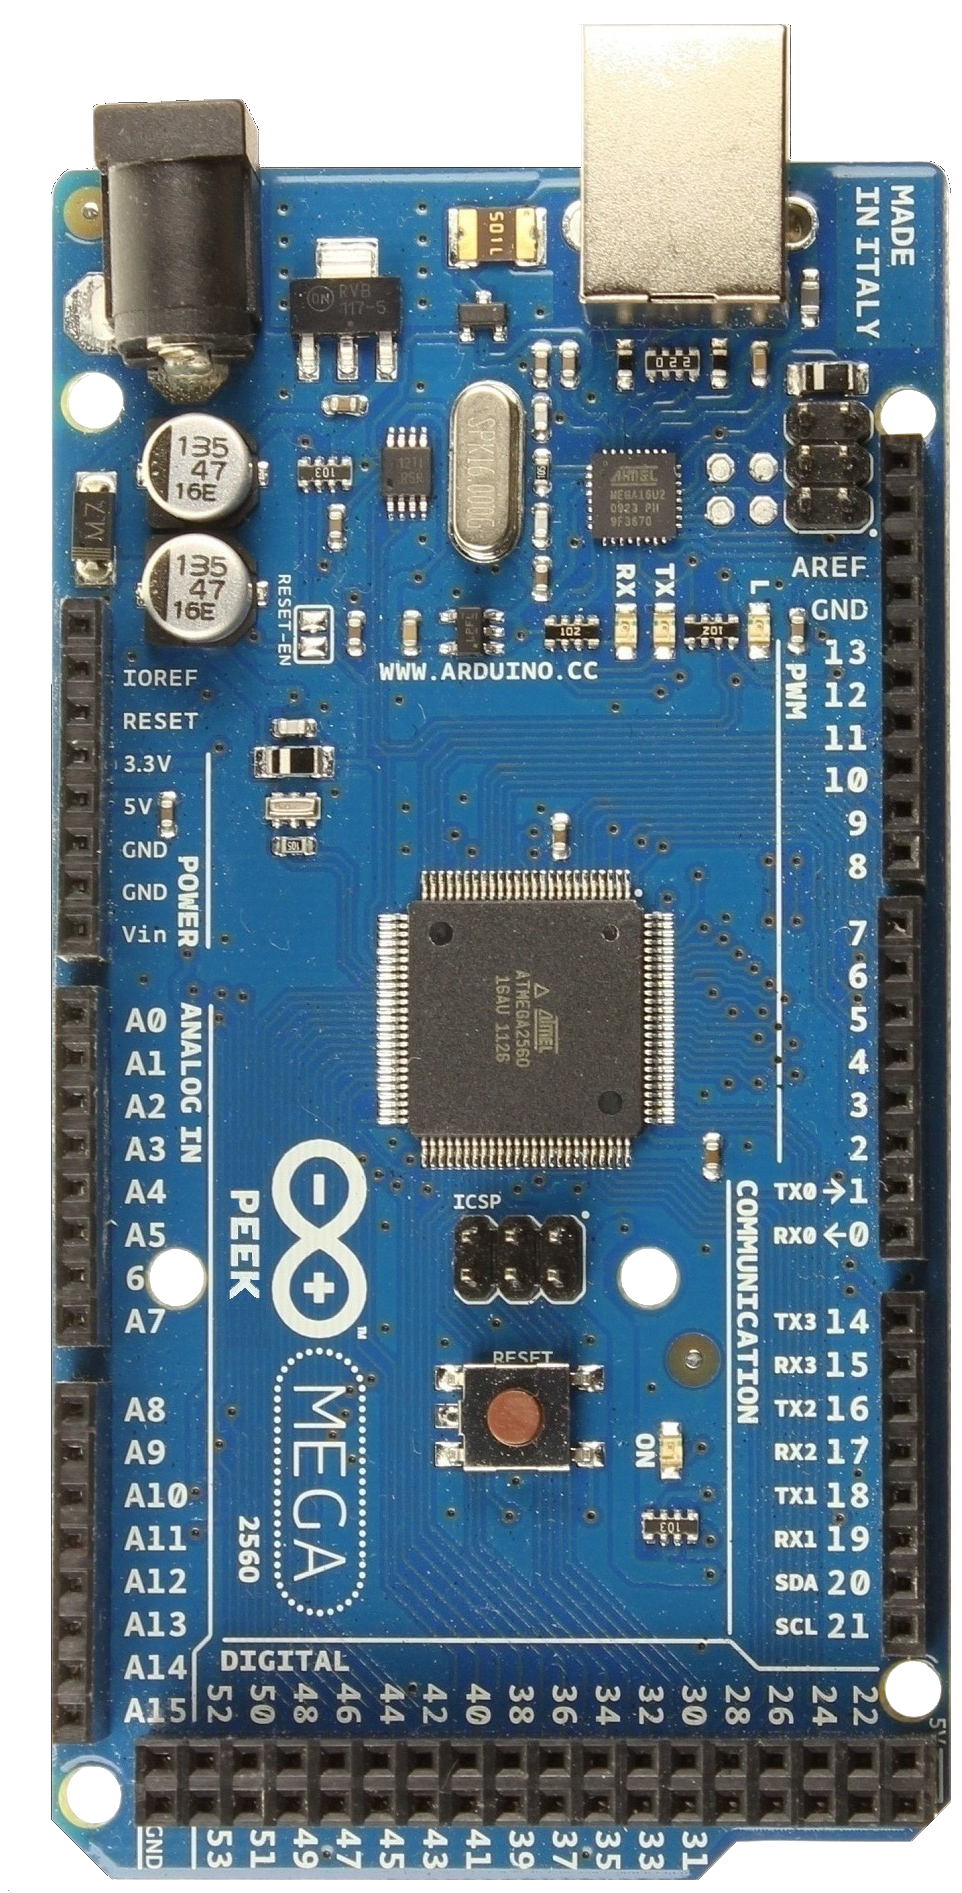
\includegraphics[width = 0.9\textwidth]{billeder/arduinoMega2560.png}
		\caption{Arduino Mega 2560}\label{fig:arduinoMega2560}
	\end{figure}
\end{minipage}\\

Den lave mængde af Ramdom Acces Memmory (RAM), umuliggør at sample hele signalet fra tryksensoren til hukommelsen, som det ses på figur \ref{fig:OscillometriskMetode}. Dette umuliggør signalbehandling af hele signalet. Prototypen sampler derfor kun toppunkterne på det oscillerende signal til hukommelsen og databehandler derefter på disse samples. Den lave mængde af samples udelukker en mere avanceret og tung digital signal behandling.

Analog Digital Converter'en (ADC) på 10 bit kræver på grund af sin lave opløsning et analogt støttekredsløb, for at kunne måle de små ændringer i trykket, som det pulserende signal er. Det analoge kredsløb sænker fleksibiliteten af prototype udviklingen, på grund af den ekstra arbejdsbyrde, det kræver at tilføre ændringer til et sådan kredsløb.

8-Bit Microcontrolleren tager mange cykluser om at regne med float tal, og har derfor begrænset udviklingsprocessen fordi der hele tiden skal optimeres i softwaren, for at udregninger ikke skal tage for lang tid at udføre.


\subsection{Udseende}
Designet af kassen, som skal indeholde alle delelementerne af prototypen, som er beskrevet i kravspecifikationen (Se de ikke-funktionelle krav under udviklingsdokumentationen), er ikke blevet implementeret på grund af tidspres. Afgrænsningen fra et godt udseende til fordel for funktionalitet og brugervenlighed blev besluttet med baggrund i at \textit{konditioneringsapparatet} er en prototype, som ikke skal sælges, men mere et proof of concept produkt. 
